%%%%%%%%%%%%%%%%%%%%%%%%%%%%%%%%%%%%%%%%%%%%%%%%%%%%%%%%%%%%%%%%%%%%%%%%%%%%%%%%%%%%%%%%%%%%%%%%%%%%%%%%%%%%%%%%%%%%%%%%%%%%%%%%%%%%%%%%
% This is just a template to use when submitting manuscripts to Frontiers, it is not mandatory to use frontiers.cls nor frontiers.tex  %
%%%%%%%%%%%%%%%%%%%%%%%%%%%%%%%%%%%%%%%%%%%%%%%%%%%%%%%%%%%%%%%%%%%%%%%%%%%%%%%%%%%%%%%%%%%%%%%%%%%%%%%%%%%%%%%%%%%%%%%%%%%%%%%%%%%%%%%%

\documentclass{frontiersSCNS} % for Science articles
%\documentclass{frontiersMED} % for Medicine articles

\usepackage{url}

%\usepackage{lineno}
\usepackage{todonotes}
\usepackage{listings}
\lstset{language=python,
        basicstyle=\ttfamily,
        frame=single,xleftmargin=\fboxsep,xrightmargin=-\fboxsep}

% Absolute numerotation for figures
\usepackage{caption}
\usepackage{subcaption}
\usepackage{overpic}
\captionsetup{figurewithin=none}  
\captionsetup{tablewithin=none}
%\usepackage[tight]{subfigure}
\def\subfigbottomskip{0pt}

\makeatletter
% Space between floats
%\setlength\floatsep    {4\p@}
% Space between floats and text
%\setlength\textfloatsep{4\p@}
% Space above and below an inline figure
%\setlength\intextsep   {4\p@}
\makeatother


\newcommand{\alex}[1]{\todo[inline, color=green!40]{#1}}
\newcommand{\fabian}[1]{\todo[inline, color=blue!40]{#1}}



%\linenumbers


\copyrightyear{}
\pubyear{}
%\onecolumn
%%% write here for which journal %%%
\def\journal{Neurosciences}
\def\DOI{}
\def\articleType{}
\def\citing{\color{darkgray}\cite}
\def\keyFont{\fontsize{6}{11}\helveticabold }
\def\firstAuthorLast{Alexandre Abraham {et~al}} %use et al only if is more than 1 author

% XXX Review the order of authors

\def\Authors{
    Alexandre Abraham\,$^{1,2,*}$,
    Fabian Pedregosa\,$^{1,2}$,
    Michael Eickenberg\,$^{1,2}$,
    Philippe Gervais\,$^{1,2}$,
    Andreas Muller,
    Jean Kossaifi,
    Alexandre Gramfort\,$^{1,2,3}$,
    Bertrand Thirion\,$^{1,2}$
    and Ga\"el Varoquaux\,$^{1,2}$}
% Affiliations should be keyed to the author's name with superscript numbers and be listed as follows: Laboratory, Institute, Department, Organization, City, State abbreviation (USA, Canada, Australia), and Country (without detailed address information such as city zip codes or street names).
% If one of the authors has a change of address, list the new address below the correspondence details using a superscript symbol and use the same symbol to indicate the author in the author list.
\def\Address{
    $^{1}$Parietal Team, INRIA Saclay-\^{I}le-de-France, Saclay, France\\
    $^{2}$Neurospin, I\textsuperscript{2}BM, DSV, CEA, 91191 Gif-Sur-Yvette, France\\
    $^{3}$Institut Mines-Telecom, Telecom ParisTech, CNRS LTCI, 75014 Paris, France}

% The Corresponding Author should be marked with an asterisk
% Provide the exact contact address (this time including street name and city zip code) and email of the corresponding author
\def\corrAuthor{Alexandre Abraham}
\def\corrAddress{Parietal Team, INRIA Saclay-\^{I}le-de-France, Saclay, France}
\def\corrEmail{alexandre.abraham@inria.fr}

% \color{FrontiersBlue} Is the blue color, used in the Journal name, in the title, and the names of the sections

% Bunch of code for 3D cubes

\usepackage{tikz}
\usetikzlibrary{calc, spy}
\usepackage{adjustbox}
% Three counters
\newcounter{x}
\newcounter{y}
\newcounter{z}

% The angles of x,y,z-axes
\newcommand\xaxis{210}
\newcommand\yaxis{-30}
\newcommand\zaxis{90}

% The top side of a cube
\newcommand\topside[3]{
  \fill[fill=white!50!blue, opacity=.9, draw=black, line width=.8pt,shift={(\xaxis:#1)},shift={(\yaxis:#2)},
  shift={(\zaxis:#3)}] (0,0) -- (30:1) -- (90:1) --(150:1)--(0,0);
}

% The left side of a cube
\newcommand\leftside[3]{
  \fill[fill=white!80!blue, opacity=.9, draw=black, line width=.8pt, shift={(\xaxis:#1)},shift={(\yaxis:#2)},
  shift={(\zaxis:#3)}] (0,0) -- (0,-1) -- (210:1) --(150:1)--(0,0);
}

% The right side of a cube
\newcommand\rightside[3]{
  \fill[fill=white!30!blue, opacity=.9, draw=black, line width=.8pt,shift={(\xaxis:#1)},shift={(\yaxis:#2)},
  shift={(\zaxis:#3)}] (0,0) -- (30:1) -- (-30:1) --(0,-1)--(0,0);
}

% The cube 
\newcommand\cube[3]{
  \topside{#1}{#2}{#3 - 1} \leftside{#1 - 1}{#2}{#3} \rightside{#1}{#2 - 1}{#3}
  \topside{#1}{#2}{#3} \leftside{#1}{#2}{#3} \rightside{#1}{#2}{#3}
}

% Example of table from template

% \begin{table}[!t]
% \processtable{Resolution Requirements for the figures\label{Tab:01}}
% {\begin{tabular}{lllll}\toprule
% Image Type & Description & Format & Color Mode & Resolution\\\midrule
% Line Art & An image composed of lines and text,  & TIFF, EPS, JPEG & RGB, Bitmap & 900 - 1200 dpi\\
%            & which does not contain tonal or shaded areas.& & &\\
%            Halftone & A continuous tone photograph, which contains no text. & TIFF, EPS, JPEG & RGB, Grayscale & 300 dpi\\
% Combination & Image contains halftone + text or line art elements. & TIFF, EPS, JPEG & RGB,Grayscale & 600 - 900 dpi\\\botrule
% \end{tabular}}{This is a footnote}
% \end{table}


% Figures

% \textbf{Figure 1.}{ Enter the caption for your figure here.  Repeat as  necessary for each of your figures.}\label{fig:01}
% Don't add the figures in the LaTeX files, please upload them when submitting the article. Frontiers will add the figures at the end of the provisional pdf.


%%%%%%%%%%%%%%%%%%%%%%%%%%%%%%%%%%%%%%%%%%%%%%%%%%%%%%%%%%%%%%%%%%%%%%%%%%%%%%%
%%%%%%%%%%%%%%%%%%%%%%%%%%%%%%%%%%%%%%%%%%%%%%%%%%%%%%%%%%%%%%%%%%%%%%%%%%%%%%%
%%%%                                                                       %%%%
%%%%                          Naming convention                            %%%%
%%%%                                                                       %%%%
%%%%%%%%%%%%%%%%%%%%%%%%%%%%%%%%%%%%%%%%%%%%%%%%%%%%%%%%%%%%%%%%%%%%%%%%%%%%%%%
%%%%%%%%%%%%%%%%%%%%%%%%%%%%%%%%%%%%%%%%%%%%%%%%%%%%%%%%%%%%%%%%%%%%%%%%%%%%%%%

% Nifti world
% -----------
% - func_filename: name of a dataset file
% - func_img: name of a (loaded) nifti file
% - func_data, func_affine: data and affine of functional data

% Scikit-learn world
% ------------------
% - Xs: list of unmasked func_data (scikit-learn world)
% - X: unmasked func_data reduced to 2 dimensions (scikit-learn world)
% - y: labels

\begin{document}
\onecolumn
\firstpage{1}

\title[Machine Learning for Neuroimaging with Scikit-Learn]{Machine Learning for Neuroimaging with Scikit-Learn}
\author[\firstAuthorLast ]{\Authors}
\address{}
\correspondance{}
\editor{}
\topic{Research Topic}

\maketitle
\begin{abstract}

\section{}
Statistical machine learning methods are increasingly used for
neuroimaging data analysis. Their main virtue for this type of application
is their ability to model high-dimensional datasets, e.g.\ multivariate
analysis of activation images, or capturing inter-subject variability.
Supervised learning is typically used in \emph{decoding} or
\emph{encoding} settings to relate
brain images to behavioral or clinical observations, while
unsupervised learning is typically used to uncover hidden structure in
sets of images (e.g.\ resting state functional MRI) or to find
sub-populations in large cohorts of subjects. By considering
functional neuroimaging use cases, we illustrate how scikit-learn,
a Python machine learning library, can be used to perform some key
analysis steps. Scikit-learn contains a large set of statistical
learning algorithms, both supervised and unsupervised, that can be applied
to neuroimaging data after a proper preprocessing. Combined with other
Python libraries, neuroimaging data can be loaded, processed and the results
can be visualised easily.



\tiny
% XXX Fix keywords
%All article types: you may provide up to 8 keywords; at least 5 are mandatory.
\section{Keywords:} machine learning, statistical learning, neuroimaging,
scikit-learn, Python
\end{abstract}


\section{Introduction}

Statistical machine learning is gaining interest in
neuroimaging data analysis. It is used by neuroscientists,
who use machine learning methods as black boxes, and computer scientists,
who acquire neuroscientific knowledge on the job. This paper aims to fill 
the gap between machine learning and neuroimaging by demonstrating how a 
general-purpose machine-learning toolbox can be used to produce scripts 
for neuroimaging analysis with state-of-the-art methods
that are fully understood by both worlds.

With its mature scientific stack, Python is a growing contender in the
landscape of neuroimaging data analysis with tools such as Nipy
\citep{millman2007analysis} or Nipype \citep{gorgolewski2011} and some
frameworks for multi-variate pattern analysis already exists
\citep{hanke2009pymvpa}. 

In this paper, we show how scikit-learn, a Python machine learning
library \citep{pedregosa2011}, can
be used on neuroimaging data. Through three use cases, we describe how to
resolve common neuroimaging problems, which method should be use and why, and how to
get the desired results. We discuss not only prediction scores, but
also the interpretability of the results, which leads us to open up the black
box methods.

\subsection{Scientific Python and neuroimaging ecosystem}

Thanks to its scientific libraries, Python is able to compete with languages
originally made for scientific computation like Matlab or R. The main libraries
are:
\begin{itemize}
    \item{\bf Scipy and Numpy} packages are the basis of scientific computing in Python.
        NumPy provides the \verb!ndarray! data type, an efficient $n$-dimensional data
        representation for array-based numerical computating, a la Matlab
        \citep{vanderwalt2011}.
        SciPy provides higher level mathematical functions that operate on ndarrays for
        a variety of domains including linear algebra, optimization and signal
        processing. Together, NumPy and SciPy provide a robust scientific environment
        for numerical computing and they are the elementary bricks we use in all our
        algorithms.

    \item{\bf Matplotlib} is a plotting library tightly integrated into the
        the scientific Python stack \citep{hunter2007}. It offers publication-quality figures in
        a variety of formats and can display plots or images in a
        graphical user interface. All figures in this paper have been generated using
        it.

    \item{\bf Nibabel} loads ors save data in popular neuroimaging file format.
        It is the starting point of all our scripts.
\end{itemize}

\section{Scikit-learn}
\label{scikitlearn}

{\em Scikit-learn} \citep{pedregosa2011} is an open source machine
learning library for the Python programming language. The ambition of the
project is to provide efficient and well-established machine learning tools within
a programming environment that is accessible to non-machine learning experts
and reusable in various scientific areas.

\subsection{Concepts}

In {\em scikit-learn}, all objects and algorithms accept data represented
in a generic domain-independent 2-dimensional array, samples $\times$
features. Scikit-learn objects share a uniform set of methods that
depends on their purpose: \textit{estimators} can build and fit models,
\textit{predictors} can make predictions and \textit{transformers}
converting data from one representation to another.

\begin{itemize}
\item {\bf Estimator}. The \textit{estimator} interface, the core of the
    library, exposes a \texttt{fit} method for learning a model from training data.
    All supervised
    and unsupervised learning algorithms (e.g., for classification, regression or
    clustering) are offered as objects implementing this interface. Machine
    learning tasks such as feature extraction, feature selection or dimensionality
    reduction are also provided as estimators.

\item {\bf Predictor}. The \textit{predictor} interface extends the notion of an estimator
    by adding a \texttt{predict}
    method that takes an array \texttt{X\_test} and produces
    predictions for \texttt{X\_test}, based on the learned parameters of the
    estimator (we call the input to \texttt{predict} ``\texttt{X\_test}'' in order
    to emphasize that \texttt{predict} generalizes to new data). In the case of
    supervised learning estimators, this method typically returns the predicted
    labels or values computed by the model.

\item {\bf Transformer}. As it is common to modify or filter data before feeding it to a learning
    algorithm, some estimators in the library implement a \textit{transformer}
    interface which defines a \texttt{transform} method. Preprocessing, feature selection and
    dimensionality reduction
    algorithms are all provided as transformers within the library. If the transformation
    can be inverted, a method called \verb!inverse_transform! also exists.

\end{itemize}

\subsection{Model selection and cross validation}

The problem of model selection is to find the best
combination of hyper-parameters with respect to some user-specified criterion,
most often the prediction score on unseen data.

In {\em scikit-learn}, model selection is supported in two distinct
estimators, \texttt{GridSearchCV}. It takes
as input an estimator, whose hyper-parameters must be
optimized, and a set of hyperparameter settings to search through. This set is
represented as a mapping of parameter names to a set of discrete choices in
the case of grid search, which exhaustively enumerates the ``grid'' (cartesian
product) of complete parameter combinations.

\section{From MR volumes to a data matrix}

From this point, it is supposed that common MRI preprocessings have been applied
to the data (namely motion correction, slice timing, coregistration on a common template like
MNI if necessary). Reference softwares for this task are
SPM\footnote{http://www.fil.ion.ucl.ac.uk/spm}~\citep{friston2007} and
FSL\footnote{http://fsl.fmrib.ox.ac.uk}~\citep{smith2004}. A python interface to
these tools is available in nipype Python library \citep{gorgolewski2011}.
This section deals with transforming neuroimaging data into a format that can be
fed to scikit-learn's functions.


\subsection{Transformation matrix}

Neuroimaging data are represented by 4-dimensional data (3D scans composed of
voxels and their associated time series) along with a transformation matrix
(called affine) used to compute voxel locations from voxel coordinates to
world coordinates.
Such matrix is needed because data may be anisotropic: the distance between
two voxels is not the same depending on the direction.
This information is used by algorithms relying on the geometric structure of the
data (e.g. Searchlight).

Going from
numpy indexing \verb!array[i, j, k]! to real coordinates $(x, y, z) \in
\mathbb{R}^3$ is a simple matrix product. For example, if your transformation
matrix is diagonal (with an offset):

\[
    \begin{bmatrix}
        r_x & 0   & 0   & o_x \\
        0   & r_y & 0   & o_y \\
        0   & 0   & r_z & o_z \\
        0   & 0   & 0   & 1   \\
    \end{bmatrix}
    \begin{bmatrix}
        i \\
        j \\
        k \\
        1 \\
    \end{bmatrix}
    =
    \begin{bmatrix}
        x \\
        y \\
        z \\
        1 \\
    \end{bmatrix}
\]

% Too much information here.

% We can write a Python helper function to transpose coordinates of a mask into
% its original space:

% \begin{lstlisting}
% def get_real_world_coordinates(mask, affine):
%     # get coordinates of non zero voxels
%     mask_coords = np.where(mask != 0)
%     # add an extra dimension for the offset
%     mask_coords = mask_coords + (np.ones(len(mask_coords[0])),)
%     # apply the transformation
%     mask_coords = np.dot(affine, np.asarray(mask_coords))[:3].T
%     return mask_coords
% \end{lstlisting}

SciPy provides routines taking affine into account in its ndimage module.
When dealing with heterogeneous dataset (multiple subjects or sessions), it is
necessary to resample data upon a reference affine. This can be done using
\texttt{scipy.ndimage.affine\_transform}.

\subsection{Resampling}
\label{resampling}

Resampling consists in changing the spatial resolution of the data. This is
an interpolation and alters the data, that is why it should be used carefully.
Oversampling (increasing data resolution) leads to higher memory consumption
and computation resources with no gain in information.
Downsampling is commonly used to reduce the size of data to process.
Typical sizes are 2mm or 3mm resolutions, but the spread of high-field MR
scanner tends to lower these values.
Data scaling factor for each direction can be modified in the affine matrix.

\subsection{Signal cleaning}

Due to its acquisition process and poor resolution, neuroimaging data often has a low
signal-to-noise ratio. It contains trends and artifacts that must be removed
to ensure maximum machine learning algorithms efficiency. Signal cleaning
includes:
\begin{itemize}
    \item{\bf Detrending} removes a linear trend over the time series of each
        voxel. This is a useful step when studying fMRI data, as the voxel
        intensity itself has no meaning and we want to study its variation and
        correlation with other voxels. Detrending can be done thanks to SciPy
        (\texttt{scipy.signal.detrend}).
    \item{\bf Normalization} consists in setting the timseries variance to 1.
        This harmonization is necessary as some machine learning algorithms are
        sensible to different value ranges.
    \item{\bf Confounds removal} consists in regressing out confounding factors.
        Typical neuroimaging confounds are head movements. These spurious
        variables induce spurious correlation between all brain voxels.
        Some datasets provide estimated confounds (usually in csv files) but
        they can also be estimated (XXX: ref to compcorr).
    \item{\bf Frequency filtering} consists in removing signal which frequency is
        abnormally high or low. Low-frequency signals in fMRI data are caused by
        physiological mechanism or scanner drifts.
\end{itemize}

\subsection{Masking}

Neuroimaging data are represented in 4 dimensions: 3 dimensions for the scans,
which are positioned in a coordinate space, and one dimension for the time.
Scikit-learn algorithms, on the other hand, only accept 2-dimensional data (see
\ref{scikitlearn}).
Depending on the purpose and on the used estimator, voxels and time series can be
considered as features
or samples. For example, to reduce dimensionality of input data,
time series can be passed as features to a Principal Component Analysis.

\subsubsection{From 4-dimensional image to 2-dimensional array}

The natural way to reduce data dimension is to flatten it, losing its original
structure. A better approach draws from the fact that not all voxels in fMRI data
holds information: outer-brain voxels are of no
use and, worse, they may bring spurious noise and scanner artefacts.
A brain mask should be applied to avoid this problem. Such masks
are often given along with datasets or can be computed thanks to softwares like
FSL or SPM.\\

\begin{figure}[hbtp]
    \begin{center}
        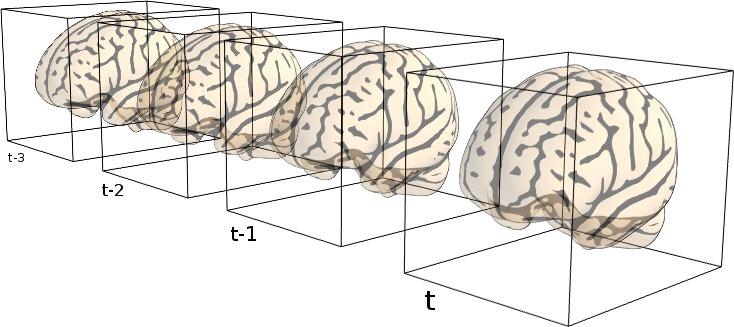
\includegraphics[width=.5\linewidth]{img/niimgs.jpg}
    \end{center}
    \caption{Conversion of brain scans into 2-dimensional data}
    \label{fig:niimg}
\end{figure}

Implementing masking procedure is made easy by NumPy fancy
indexing. Special attention must be paid to the type of the mask array: it must
be boolean. Otherwise the indexing will be considered as broadcasting and the
result will usually fill the whole memory.
2-dimensional masked data will be refered as \texttt{X} to follow scikit-learn
conventions.

\begin{lstlisting}
# Apply a mask
# Ensure that the mask is boolean
mask = mask.astype(np.bool)
# Apply the mask, X = timeseries * voxels
X = func_data[mask].T

# Unmask data
unmasked_data = np.zeros(mask.shape, dtype=X.dtype)
unmasked_data[mask] = X
\end{lstlisting}


% This part has been removed because automatic masking is overly complicated and
% does not brinautomatic masking is overly complicated and does not bring much
% to the paper.

% \subsubsection{Automatically computing a mask}

% The simplest strategy to compute a mask is a binarization by a selected threshold.
% Due to the nature of the neuroimaging data, there exists some strategy to choose
% this threshold in order to obtain a decent segmentation.

% \alex{There is a reference for the method used in Nisl. We should put it there
% and in the code. Add a figure with an histogram to illustrate.}

% Multi subject computation is simply done by intersecting subjects maps
% relatively to a chosen threshold.

\subsubsection{Label shifting}

Functional MRI acquisition is not immediate: BOLD response peak occurs between 3
and 5 seconds after the stimulus. We take this time shift into account by
shifting values of the label array by an offset of 2 time repetition (about 5
seconds).

% Functional MRI measures brain activity by using the Blood-Oxygen-Level-Dependent
% contrast (BOLD). In fact, like muscles, brain regions consume more oxygen and
% nutriments when stimulated. So when a part of the brain starts working,
% physiological mechanisms induce an oxygen-rich blood flood toward this
% particular region: this is called haemodynamic response.

% However, this reaction takes time, usually around 3-4 seconds. This is the
% duration between the event and the reaction observed in the brain. To be able to
% match these two events, we will sometimes have to shift our data. The number of
% scans that must be shifted depends on the TR (repetition time) of the data.
% Usually, we remove the first two scans of the data and the two last values of the
% labels (to keep an homogeneous length).

\begin{lstlisting}
X = X[2:]
y = y[:-2]
\end{lstlisting}

\section{Decoding object representation in the brain}

In the context of machine learning in neuroimaging, \textit{decoding} refers to learning a model
which predicts behavioral or phenotypic data given BOLD signal. It is presented
in the following use case. The inverse procedure is
called \textit{encoding} \citep{naselaris2011} and is introduced in the next use case
(section \ref{kamitani}).\\

This use case explores the relation between brain activity and visual
stimuli. More precisely, we want to know if there is a significant difference
in brain activity when presenting to the subject images of different categories.
It is based on the experiment presented in \cite{haxby2001}:
grayscale images representing different image categories
are presented to 6 subjects during 12 sessions. The goal is to predict,
from fMRI data, which image category is presented
to the subject and determine where the discriminating brain voxels for this task are
located. Full protocol information is available in the reference paper.
For the sake of simplicity, this example focuses on one subject for the
particular task of discriminating face against house images.\\

As the desired output value (face or house) is known, this problem is a
supervised learning problem. Among all methods proposed in the scikit-learn, we
chose the Support Vector Method (SVM) for this problem. In fact, it is a
reference basic algorithm which has the advantage to
give reliable results even when the number of dimensions is greater than the
number of samples.

\subsection{Feature selection: ANOVA F-Test}

The common preprocessing pipeline is applied on Haxby dataset. After masking, 40
000 features are left for only 1 400 samples. This is not an optimal setting
for machine learning algorithm which efficiency grows with the ratio
between samples and features.\\

Reducing the number of features (ie voxels) can be done by selecting the most
relevant ones to our task. A neuroscientific approach could be to restrain the
mask to occipital area which contains the visual cortex. The statistical
approach consists in using a simple and costless test to roughly reduce the
number of features, before applying a more sophisticated algorithm.\\

Scikit-learn offers a panel of strategies to select features. In supervised
learning, the most popular feature selection method is the
ANalysis Of VAriance (ANOVA) F-Test. This is a generalization of the t-test to
more than 2 features.
ANOVA compares several groups to determine if they are similar or not (the null
hypothesis being that they are randomly drawn from the same population).
It is used to compare feature distributions across classes: a feature which
distribution is similar for all classes is not likely to contain much
information.\\

After ranking the features, \verb!sklearn.feature_selection! proposes a panel
of feature selection strategies. One can choose to take a percentile of the features
(\verb!SelectPercentile!), or a fixed number of features (\verb!SelectKBest!)
for example. All these objects are implemented as transformers (see
\ref{scikitlearn}) and are invertible (see code below).
In this use case, \verb!f_classif! function (ANOVA F-Test) along with selection
of a fixed number of features will be used.

\subsection{Classification: SVM}

A Support Vector Classifier (SVC) is a simple classifier that finds a linear
hyperplane separating samples that belong to different classes. 
Classifying a new sample boils down to
seeing on which side of the hyperplane it is.
The decision is taken based upon a subset of training data called
support vectors (this is not a black box). From them, one can deduce which
features are the most important, and yield a neuroscientific interpretation out
of these results.

\begin{lstlisting}
feature_selection = SelectKBest(f_classif, k=500)
clf = SVC(kernel='linear', C=1.)
X = feature_selection.fit_transform(X)
clf.fit(X)
\end{lstlisting}

% \subsubsection{Pipeline}

% The workflow described above (feature selection + estimator) is a standard one.
% In fact, in most cases, it will consist in atomic steps
% \textit{linked} together (the output of a step is the input of the next one).
% For this purpose, scikit-learn offers a pipeline object that allows such
% linking. A pipeline is simply a list of scikit-learn objects through which the
% input data will be conveyed. The function to call for each object (transform,
% fit...) depends on its type.
% This allow developpers to create new estimators based on existing ones.

% \begin{lstlisting}
% anova_svc = Pipeline([('anova', feature_selection), ('svc', clf)])
% anova_svc.fit(X)
% sv = anova_svc.inverse_tranform(clf.support_vectors_)
% \end{lstlisting}

\subsection{Searchlight}
\label{searchlight}

Searchlight is a popular algorithm in the neuroscience community.
Presented in \cite{kriegeskorte2006}, it aims to score
brain voxels depending on the amount of information they hold. Concretely, a
cross validated SVM-based classification is run on each voxel: the better its results are,
the more information it holds.

However, considering the fact that the information of a voxel is not only
contained in the voxel itself but in its neighbourhood. Hence the Searchlight
runs the classification on a ball centered on the voxel instead of a single voxel.
It can be seen as a sophisticated version of the dimension reduction used in our
first setting.
An efficient implementation of this algorithm is way beyond the scope of this
paper also it is not detailed here. However, the code, along with this example,
are available in nilearn Python package\footnote{http://nilearn.github.io}.

\subsection{Results}

The results of this experience are shown in figure~\ref{fig:haxby}.
On all figures, green, resp.\ blue,
lines surround features corresponding to face, resp.\ house, recognition
exhibited in the reference paper.
The F-score (left) is the basic
classifier used in ANOVA to select the features. The middle pictures shows the
first support vector obtained with SVC after feature selection. The picture on
the right shows the amount of information computed by Searchlight.

First, we see that voxels selected by all methods matches the results obtained
in the original work. The F-scores are very salient, almost binary, compared to
SVC. The Searchlight highlights more voxels around the reference regions. This is
explained by the fact that its strategy to take a ball around a voxel
is similar to a blur.

These results are also neuroscientifically plausible as the activation occurs in the
high level regions of the visual cortex which is known to contain semantic
information about vision. If Searchlight only gives a score of the voxels, the
SVC allows us to classify unseen data.

\begin{lstlisting}
### Look at the discriminating weights
support = clf.support_vectors_
# reverse feature selection
support = feature_selection.inverse_transform(support)
\end{lstlisting}

\begin{figure}[hbtp]
  \begin{center}
  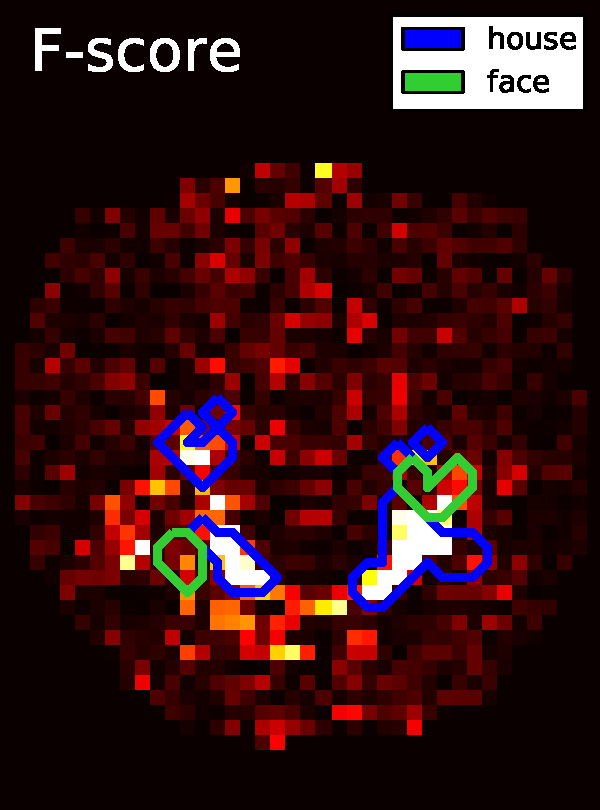
\includegraphics[width=.3\linewidth]{img/haxby/haxby_fscore}
  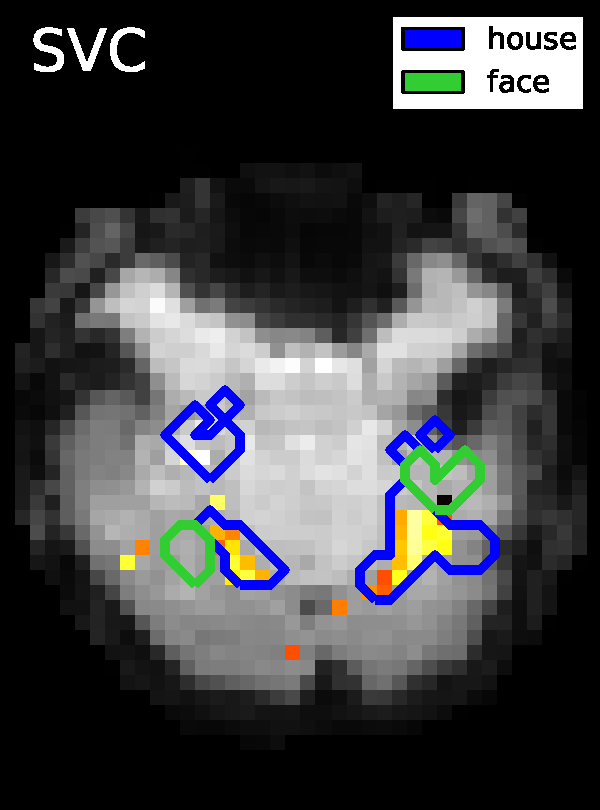
\includegraphics[width=.3\linewidth]{img/haxby/haxby_svm}
  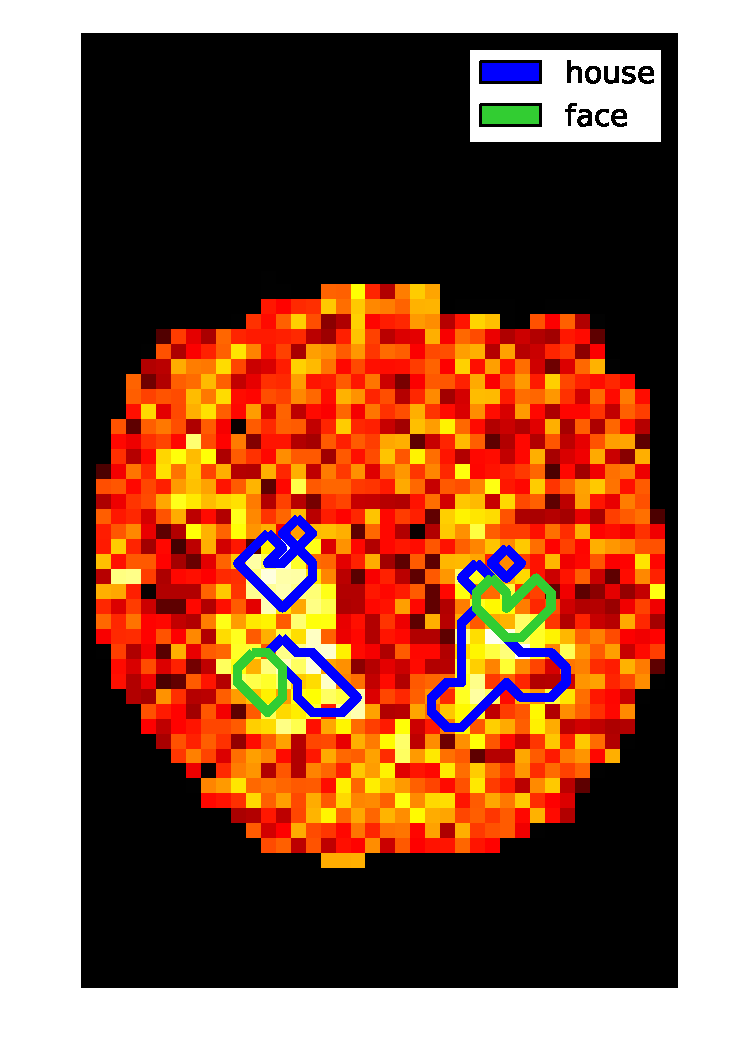
\includegraphics[width=.3\linewidth]{img/haxby/haxby_searchlight}
  \end{center}
\caption{Voxel importance in prediction decision for Haxby experiment}
\label{fig:haxby}
\end{figure}

% This is too technical
%
% \subsubsection{Implementation}
% 
% Even if this algorithm seems complicated, it can be easily implemented thanks to
% some basic bricks provided by the scikit-learn. They key elements here are
% \textit{i)} the neighbourhood (\texttt{sklearn.neighbors.NearestNeighbors}),
% \textit{ii)} the classifier (\texttt{sklearn.svm.LinearSVC}),
% \textit{iii)} the cross-validation (\texttt{sklearn.svm.LinearSVC}).
% 
% Searchlight prohibitive computational cost makes it hardly runnable on a whole
% brain. To avoid this problem, computation will be limited to voxels present in a
% \texttt{process\_mask} (in this use case, a single axial slice). This is easily
% doable thanks to scikit-learn: a connectivity graph is build upon the
% \texttt{mask} and then restricted to voxels of interest contained in the 
% \texttt{process\_mask}.
% 
% \begin{lstlisting}
% # Compute world coordinates of all in-mask voxels.
% mask_coords = get_real_world_coordinates(mask_data, mask_affine)
% 
% # Compute world coordinates of all in-processing region voxels
% process_mask_coords = get_real_world_coordinates(process_mask_data,
%                                                  process_mask_affine)
% 
% clf = neighbors.NearestNeighbors(radius=radius)
% A = clf.fit(mask_coords).radius_neighbors_graph(process_mask_coords)
% \end{lstlisting}
% 
% Then, for each row of our adjacency matrix, we do a cross validation using a
% given estimator. This is the core of the algorithm and we see that it can be
% written with a simple for-loop.
% 
% \begin{lstlisting}
% scores = np.zeros(len(A.rows))
% for i, row in enumerate(A.rows):
%     scores[i] = np.mean(
%             cross_val_score(estimator, X[:, row], y,
%                             score_func=score_func,
%                             cv=cv, n_jobs=1))
% return scores
% \end{lstlisting}
% 
% \subsubsection{Results}
% 
% Results are presented in figure \ref{fig:haxby}. Searchlight results
% (\textit{b}) are compared to the previous use case and to the F-score measure
% (\textit{c}), the simplest statistical test we can make on the data.
% All methods mainly localizes information in the region of
% interest corresponding to house detection. The smoothing effect present in the
% Searchlight results is inherent to the fact that a ball is used to iterate on
% the voxels.

\section{Encoding brain activity and decoding images}
\label{kamitani}

In the previous experiment, the category of a visual stimulus was deduced from
brain activity measured in the visual cortex.
This use case goes further by inferring a direct link between the image
seen by the subject and the brain activity.

In the experiment proposed by \citep{miyawaki2008}, several series of $10\times10$
binary images are presented to two subjects while activity on the visual cortex
is recorded.
The training set is composed of random images (where black and white pixels
are balanced) and the testing set is composed of structured images containing
geometric shapes (square, cross...) and letters. For the sake of simplicity, in
this use case, we consider only the training set and use cross-validation to
obtain scores on unseen data.\\

We will illustrate two problems: reconstructing visual stimulus from BOLD activation,
which is a decoding task, and reconstructing brain activation from visual
stimulus, which is an encoding task.

\subsection{Decoding}

Common pre-processing have been applied to the data (detrending and
standardization).

Prior knowledge on the data can help for model selection. In this experiment, we
want to find the relation between voxel activation and some pixel color. It is
therefore reasonable to suppose that not all voxels in the brain will be related to one
pixel. We will consequently use sparsity inducing models who tends to
reduce the number of features on which their decision is made.

The original work by \cite{miyawaki2008} uses a sparse multinomial
logistic regression and a sophisticated multiscale strategy to reconstruct the image.
This example uses the simpler version of this approach, a $\ell_1$ logistic
regression, and compare it to the Orthogonal
Matching Pursuit (\cite{mallat1993}). The OMP is a linear model that uses
feature time series as a dictionary and an l1 constraint on the loadings. Its
particularity is to add one atom at each step and update all coefficients
based on the orthogonal projection on previously selected atoms.
Reconstruction performance is measured by the accuracy score, the default
function proposed in the scikit-learn.

\begin{lstlisting}
from sklearn.linear_model import OrthogonalMatchingPursuit as OMP
from sklearn.cross_validation import cross_val_score

pipeline_OMP = Pipeline([('selection', SelectKBest(f_classif, 500)),
                         ('clf', OMP(n_nonzero_coefs=20)])

scores_omp = []
# y_train = n_samples x n_voxels
# To iterate on voxels, we transpose it.
for pixel in y_train.T:
    score = cross_val_score(pipeline_OMP, X_train, pixel, cv=5)
    scores_omp.append(score)
\end{lstlisting}

\subsubsection{Results}

Results are presented in figure~\ref{fig:decoding}.
Looking at both methods (figures \textit{a} and \textit{c}), we observe that reconstruction
is more accurate in the fovea, as observed in the original work \citep{miyawaki2008}.
This may be caused by the fact that there are more neurons dedicated to foveal
representation in the primary visual area than for the borders.

Comparing the two methods, we see that Logistic Regression gives better results
than Orthognal Matching Pursuit. However, LR bases its decision upon 200 voxels
while the OMP has been forced to base it on 40.

The pixel weights (\textit{b} and \textit{c}) agree on the fact that important
domains are located in the blue shape.
Both methods have selected the same voxel to base their decision upon.
This particular voxel will be studied in the encoding task in the next section.

\begin{figure}[hbtp]
  \begin{center}
    \begin{subfigure}[c]{.07\linewidth}
    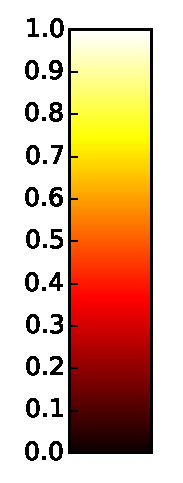
\includegraphics[width=\linewidth]{img/kamitani/score_colorbar}
    \end{subfigure}
    \begin{subfigure}[c]{.2\linewidth}
    %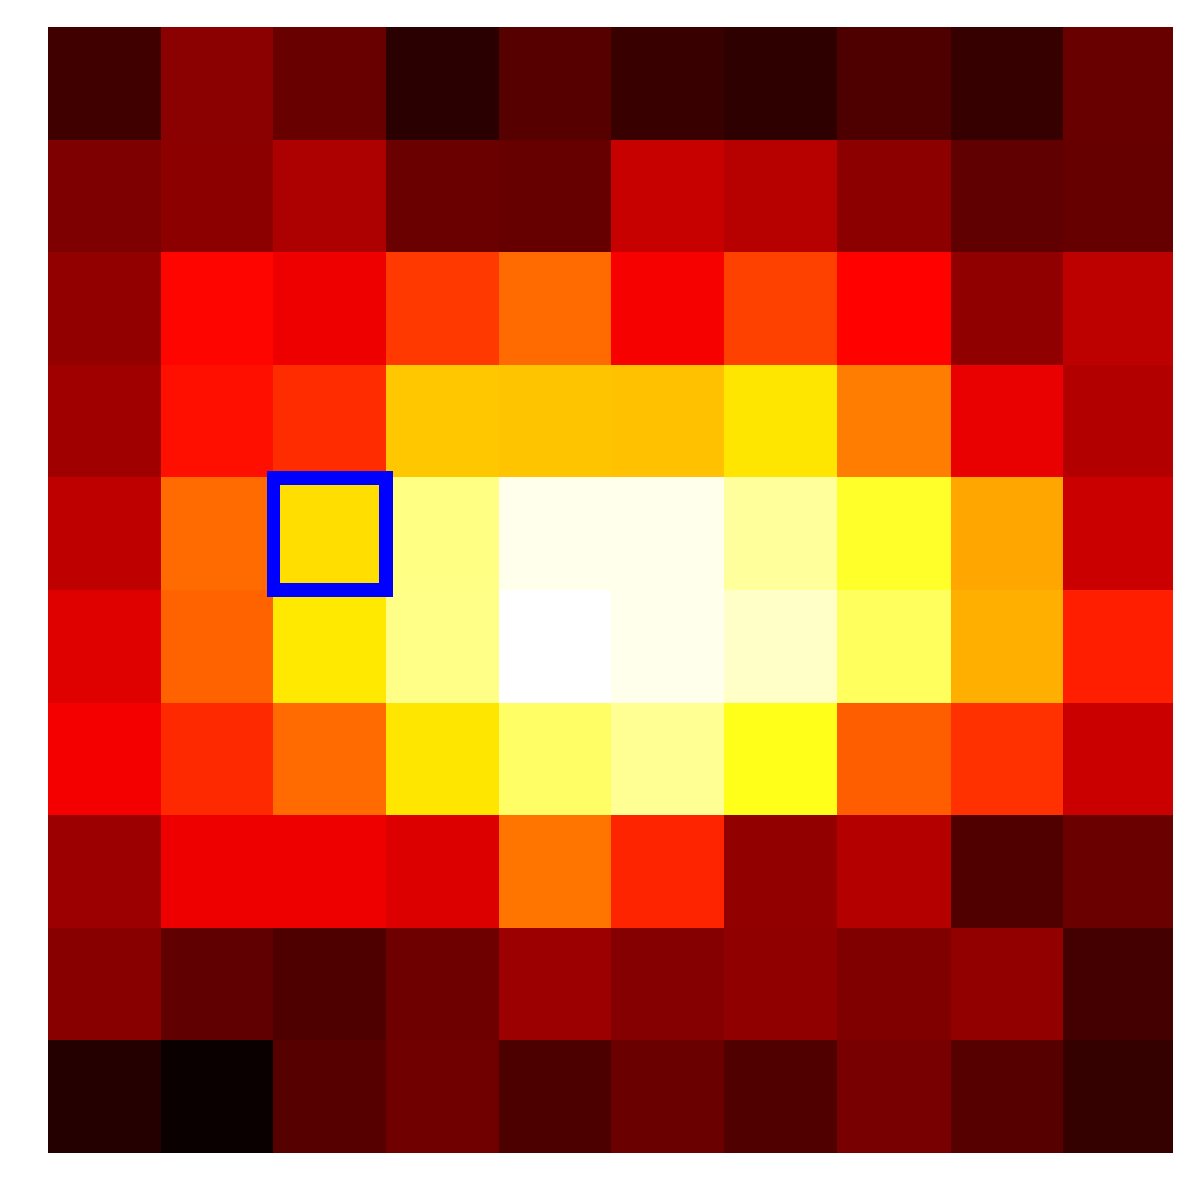
\includegraphics[width=\linewidth]{img/kamitani/scores_log}
        \begin{overpic}[width=\linewidth]{img/kamitani/scores_log}
            \put(2, 2){a}
        \end{overpic}
    %\subcaption{Logistic regression scores}
    \end{subfigure}
    \begin{subfigure}[c]{.2\linewidth}%
        \begin{tikzpicture}
          \begin{scope}[spy using outlines={blue, circle, line width=3pt,
                magnification=6, size=60, connect spies}]
            \node[inner sep=0pt, rotate=90](img){
                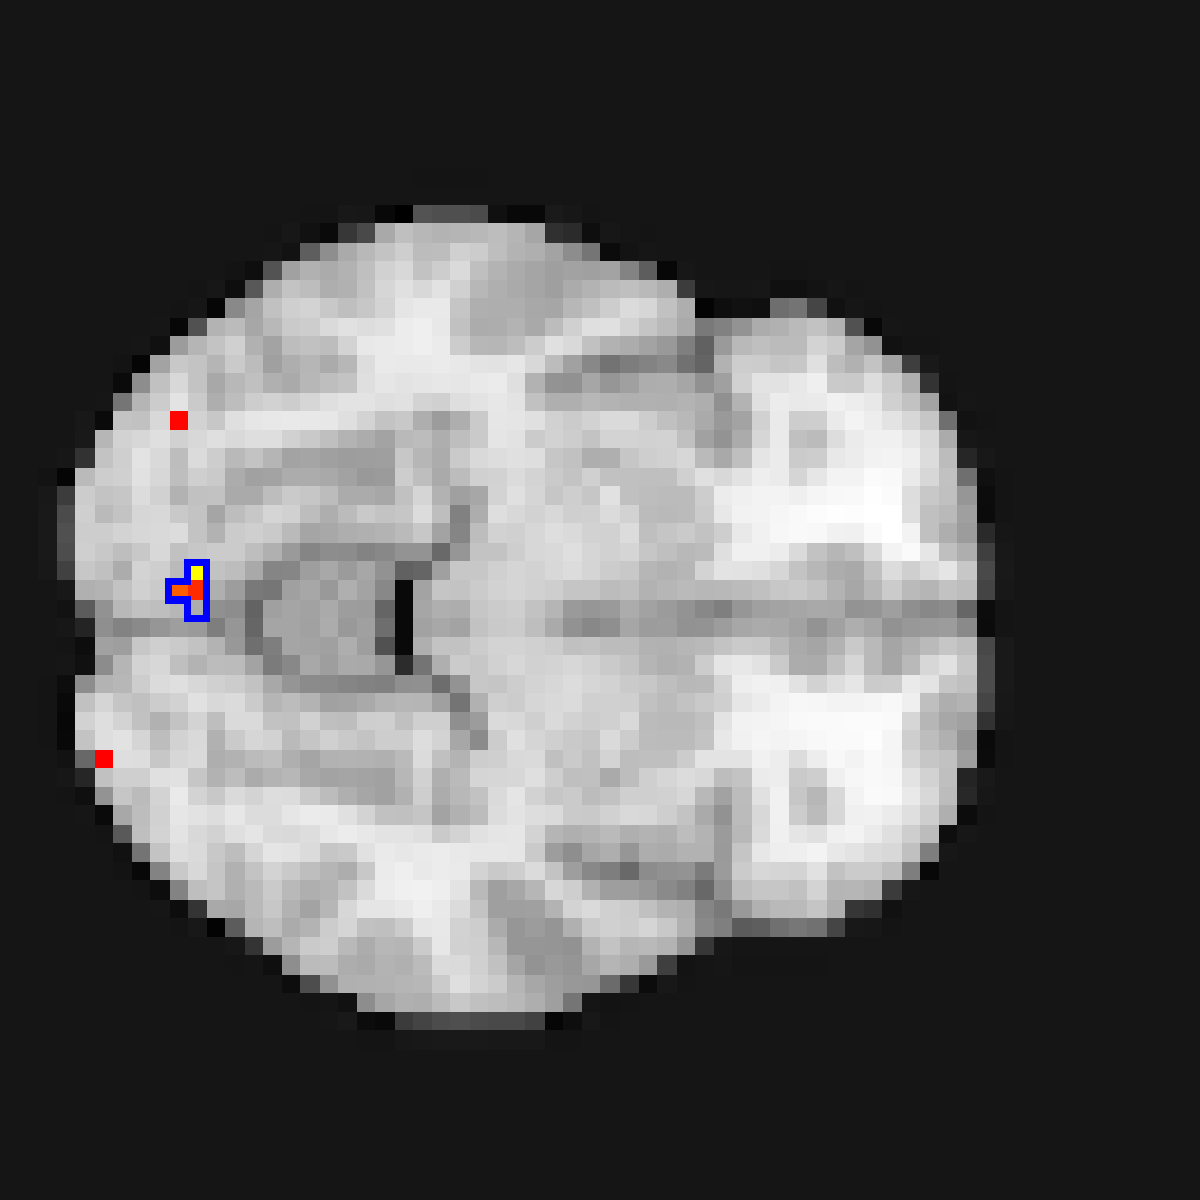
\includegraphics[width=\linewidth]{img/kamitani/pixel_logistic}};
            \node[inner sep=0pt] at (-1.6, -1.6) {\textcolor{white}{b}};
            \spy [width=2cm, height=2cm, line width=3pt, spy connection path={\draw[line
            width=2pt, blue] (tikzspyonnode) -- (tikzspyinnode);}]
            on (-0.03, -1.2) in node (a) [line width=4pt] (a) at (.6, .6) (a) {};
        \end{scope}
    \end{tikzpicture}
    %\caption{Voxel weights for logistic regression}
    \end{subfigure}
    \begin{subfigure}[c]{.2\linewidth}
    %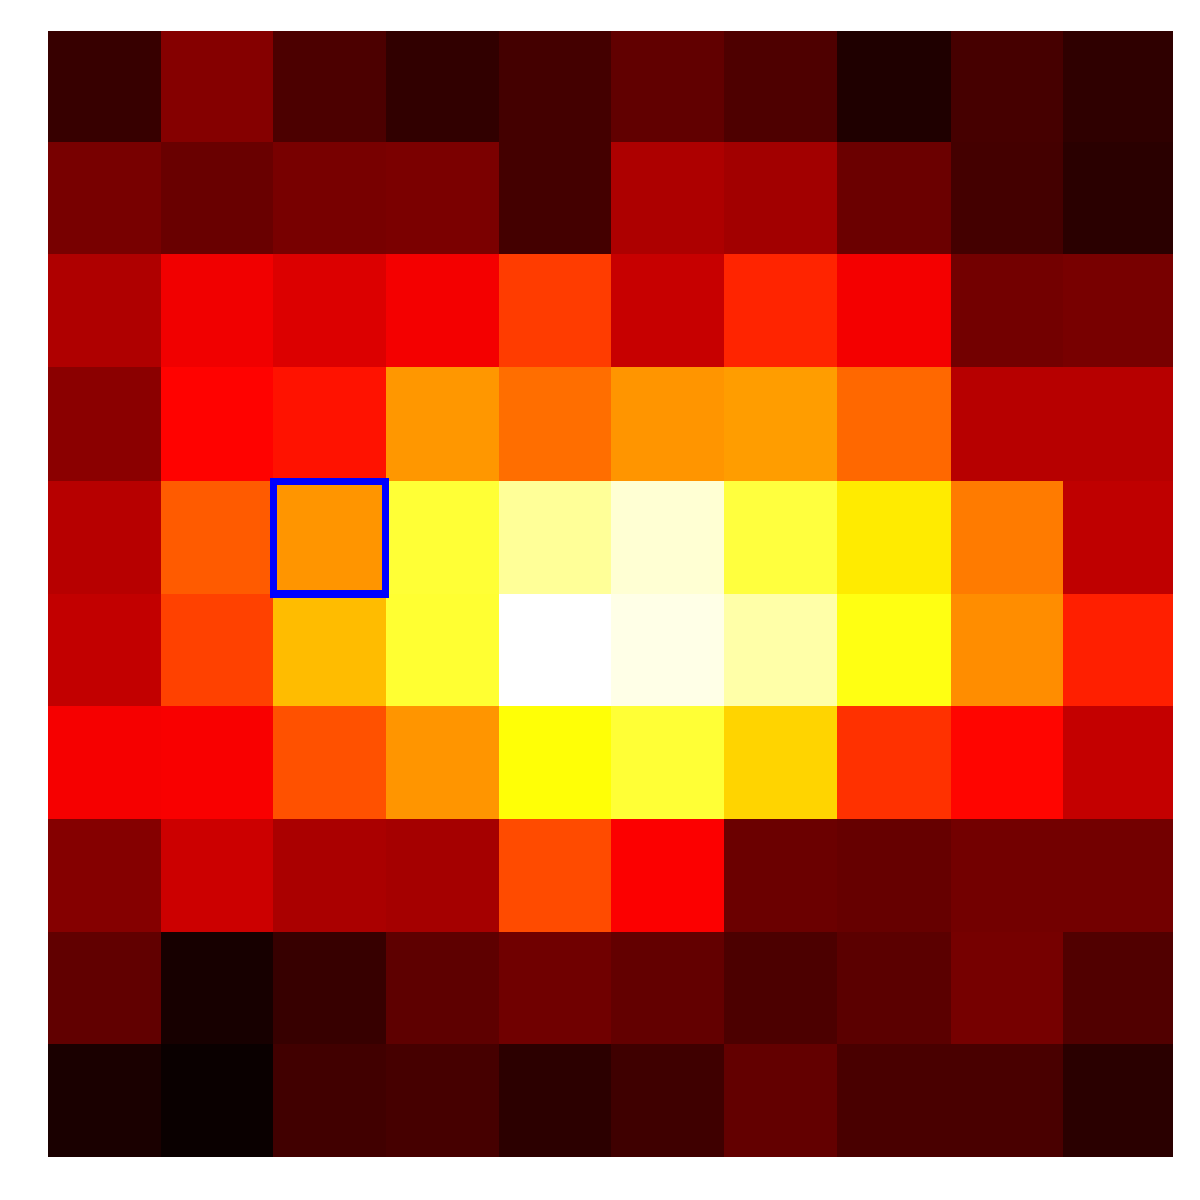
\includegraphics[width=\linewidth]{img/kamitani/scores_omp}
        \begin{overpic}[width=\linewidth]{img/kamitani/scores_omp}
            \put(2, 2){c}
        \end{overpic}
    %\caption{OMP scores}
    \end{subfigure}
    \begin{subfigure}[c]{.2\linewidth}
      \begin{tikzpicture}
          \begin{scope}[spy using outlines={blue, circle, line width=3pt,
                magnification=6, size=60, connect spies}]
            \node[inner sep=0pt, rotate=90]{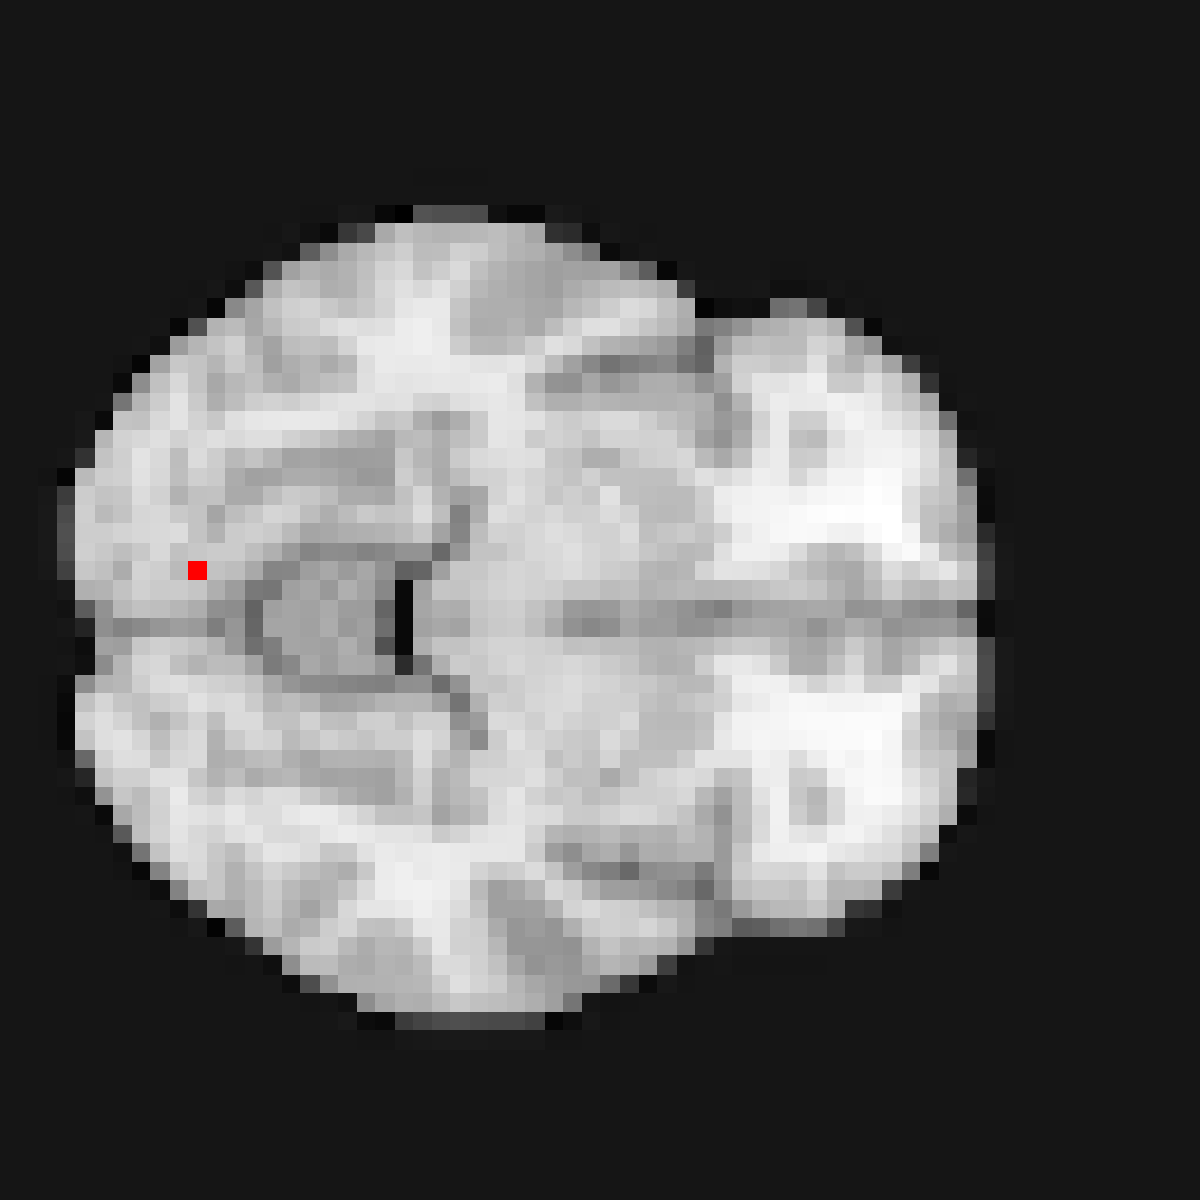
\includegraphics[width=\linewidth]{img/kamitani/pixel_omp}};
            \node[inner sep=0pt] at (-1.6, -1.6) {\textcolor{white}{d}};
            \spy [width=2cm, height=2cm, line width=3pt, spy connection path={\draw[line
            width=2pt, blue] (tikzspyonnode) -- (tikzspyinnode);}]
            on (-0.03, -1.2) in node (a) [line width=4pt] (a) at (.6, .6) (a) {};
        \end{scope}
    \end{tikzpicture}
    %\caption{Voxel weights for OMP}
    \end{subfigure}
  \end{center}
  \caption{Reconstruction accuracy per pixel depending on the method (\textit{a.} Logistic
      regression, \textit{c.} OMP). The brain voxels
  corresponds to coefficients used to predict the blue bordered pixel(\textit{b.} Logistic
      regression, \textit{d.} OMP). This
  figure should be put in relation with figure~\ref{fig:encoding}.}
\label{fig:decoding}
\end{figure}

\subsection{Encoding}
Given an appropriate model of the stimulus, e.g. one which can provide an approximately linear representation of BOLD activation, an encoding approach allows one to quantify for each voxel to what extent its variability is captured by the model. A popular evaluation method is the predictive \(r^2\) score, which uses a prediction on left out data to quantify the decrease in residual norm brought about by fitting a regression function as opposed to fitting a constant. %We have \[r^2 = \frac{\|y_{\textrm{true}} - y_{\textrm{pred}}\|^2}{\|y_{\textrm{true}} - \bar y_{\textrm{true}}\|^2}\]
The remaining variance consists of potentially unmodelled, but reproducible signal and spurious noise.

On the Kamitani dataset, we can observe that mere black and white pixel values can explain a large part of the BOLD variance in many visual voxels. Sticking to the notation that \(X\) represesents BOLD signal and \(y\) the stimulus, we can write an encoding model using the ridge regression estimator of the scikit-learn:

\begin{lstlisting}
from sklearn.linear_model import Ridge
from sklearn.cross_validation import KFold

cv = KFold(len(y_train), 10)
# Fit ridge model, calculate predictions on left out data
# and evaluate r^2 score for each voxel
scores = []
for train, test in cv:
    pred = (Ridge(alpha=100.).fit(y_train[train], X_train[train])
                             .predict(y_train[test]))
    X_true = X_train[test]
    scores.append(
        1. - ((X_true - pred) ** 2).sum(axis=0) /
        ((X_true - X_true.mean(axis=0)) ** 2).sum(axis=0))
    
mean_scores = np.array(scores).mean(axis=0)
\end{lstlisting}

\subsubsection{Results}
The variable \texttt{mean\_scores} contains a score for each voxel. Visualized in a brain volume we obtain figure \ref{fig:encoding}, in which we can observe that the BOLD signal especially in early visual areas, most notably V1, is very well explained as a linear function of the pixel intensities, with a predictive score of up to \(r^2 = 0.6\).

\subsubsection{Receptive fields}
Given the retinotopic structure of early visual areas, we are led to expect their voxels to have strongly localized so-called population receptive fields (\textit{prf}). This suggests that per voxel only very few stimulus pixels should suffice to explain its activity. This information can be exploited by using a sparse coding approach to find the receptive fields.

\begin{lstlisting}
from sklearn.linear_model import LassoLarsCV

# choose number of voxels to treat, set to None for all voxels
n_voxels = 50
# choose best voxels
indices = mean_scores.argsort()[::-1][:n_voxels]

lasso = LassoLarsCV(max_iter=10)

receptive_fields = [lasso.fit(y_train, X_train[:, index]
        ).coef_.reshape(10, 10)
        for index in indices]

\end{lstlisting}
%y_train_centered = (y_train - y_train.mean(axis=0)) / y_train.std(axis=0)

Receptive fields are show on the right part of figure~\ref{fig:encoding}. We can
see that receptive fields of neighboring voxels are neighbouring pixels, which
is an expected result as we know that primary visual cortex direclty encodes
visual stimuli. Moreover, we note that our two approaches give matching results 
to the voxel.

\begin{figure}[hbtp]
  \begin{center}
    \begin{tikzpicture}
        \begin{scope}[spy using outlines={blue, circle, line width=3pt,
                magnification=6, size=60, connect spies}]
                \node[rotate=90] {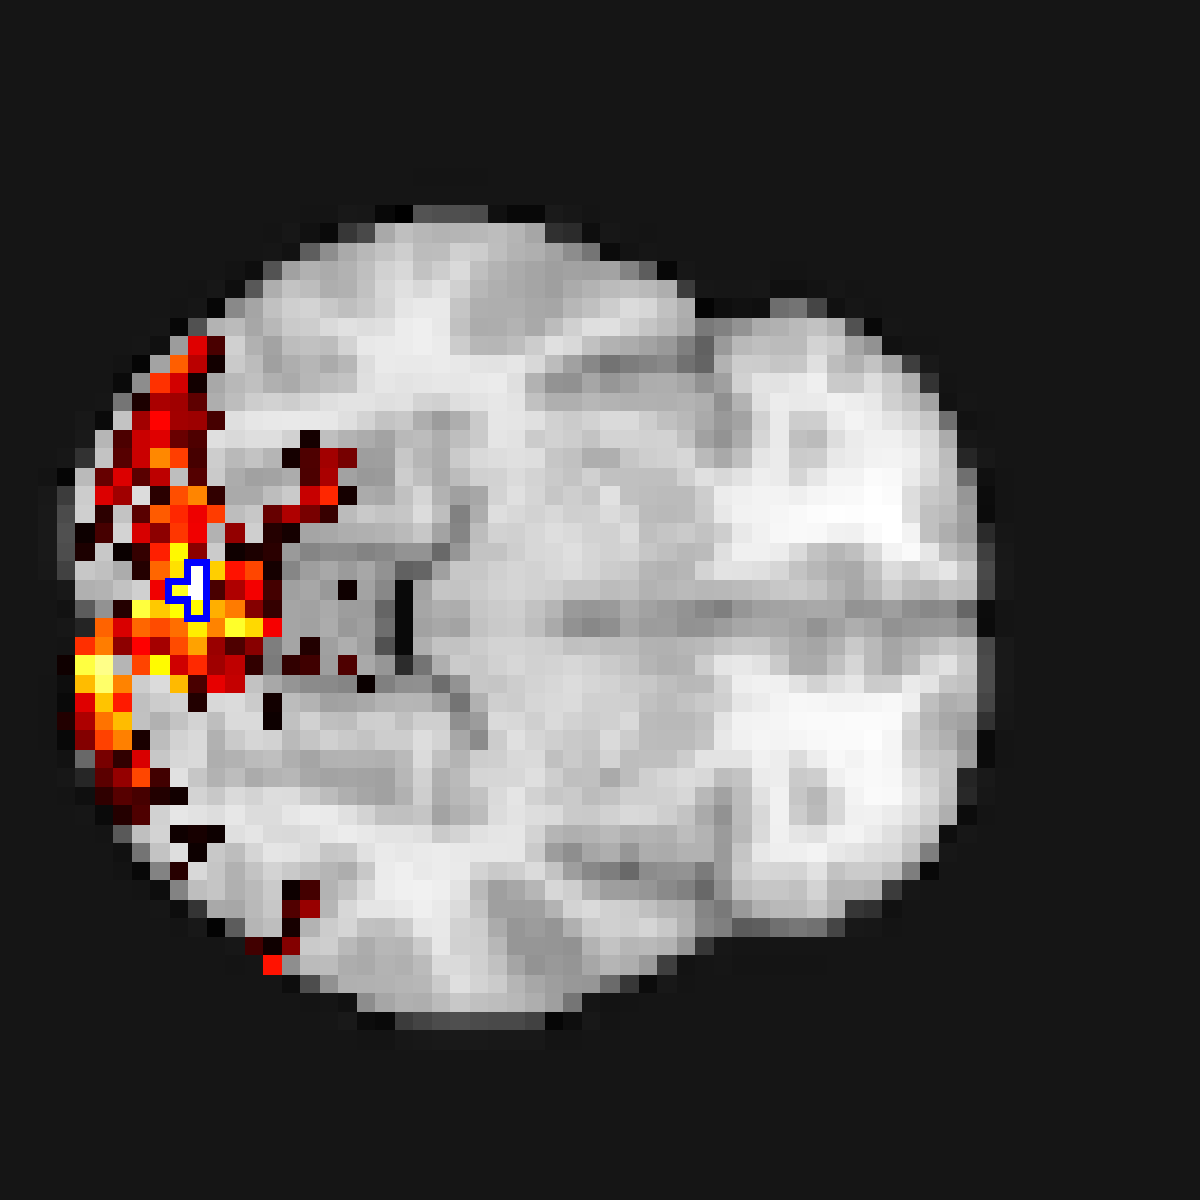
\includegraphics[width=5cm]{img/kamitani/encoding_scores}};
            \spy [width=3cm, height=3cm, line width=3pt, spy connection path={\draw[line
            width=2pt, blue] (tikzspyonnode) -- (tikzspyinnode);}]
            on (-0.04, -1.7) in node (a) [line width=4pt] (a) at (1.2,1) (a) {};
        \end{scope} 

        \node (i1780) at (4.4, 1.3)
            {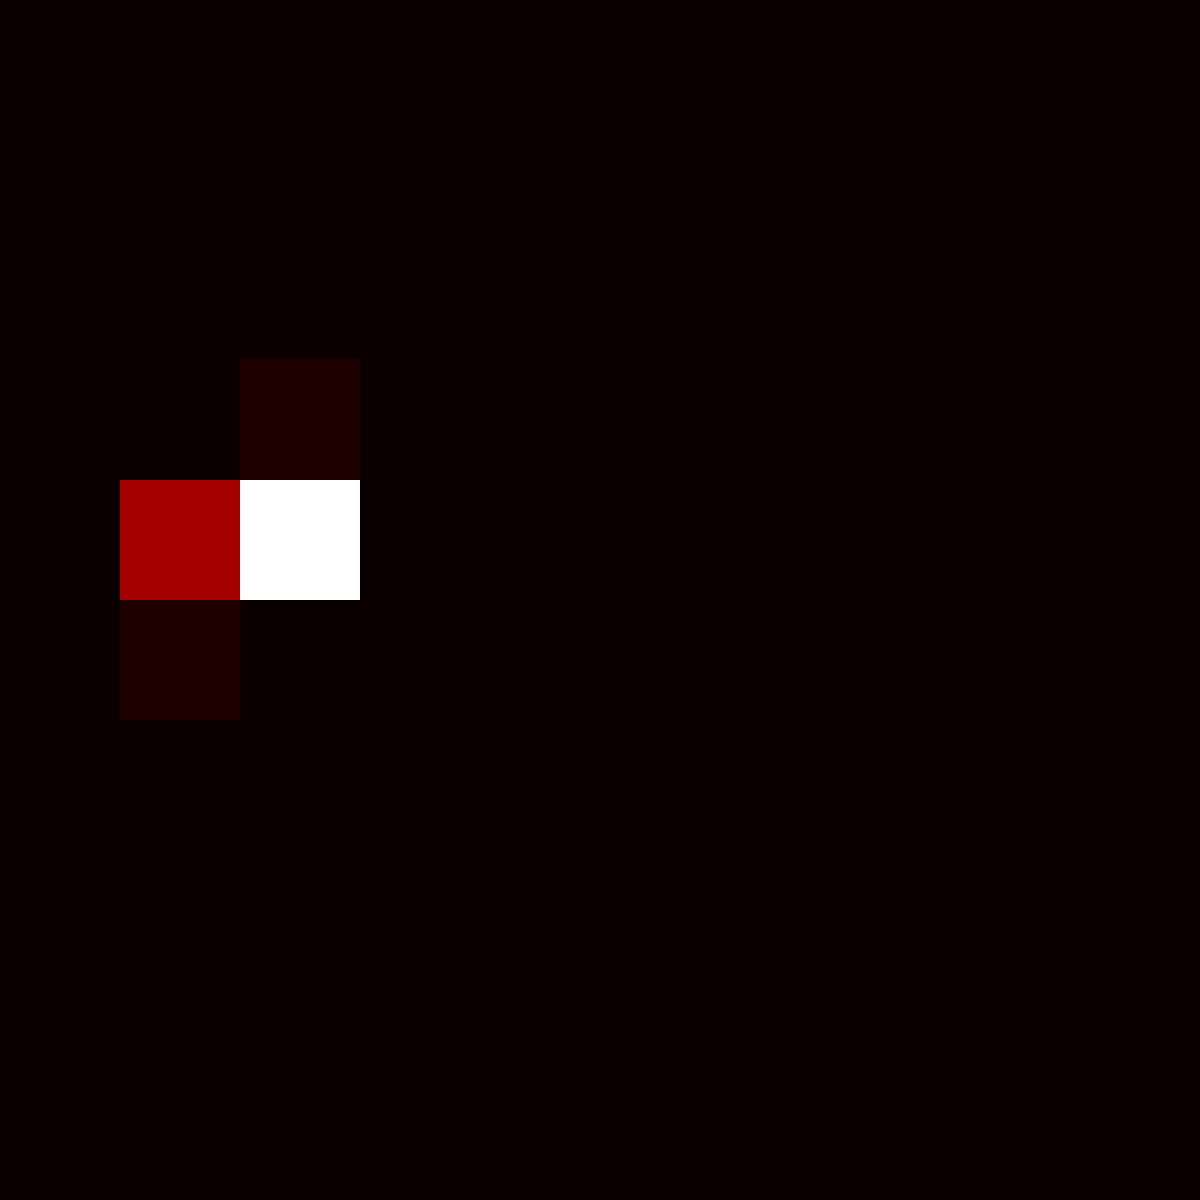
\includegraphics[width=2.4cm]{img/kamitani/encoding_1780}};
        \node (i1951) at (7, 1.3)
            {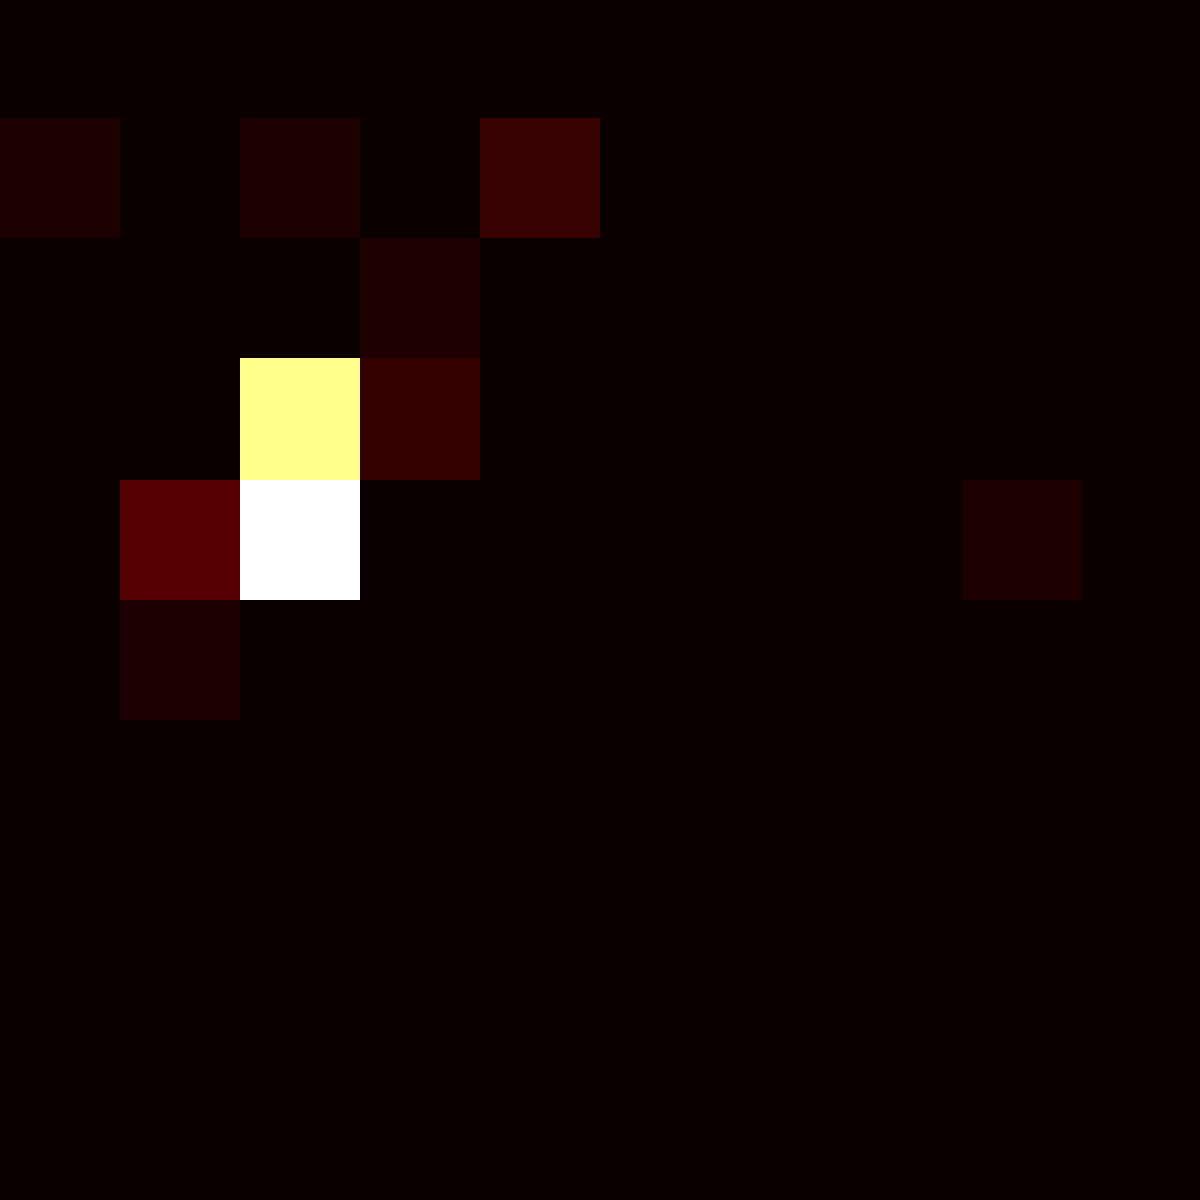
\includegraphics[width=2.4cm]{img/kamitani/encoding_1951}};
        \node (i2131) at (9.6, 1.3)
            {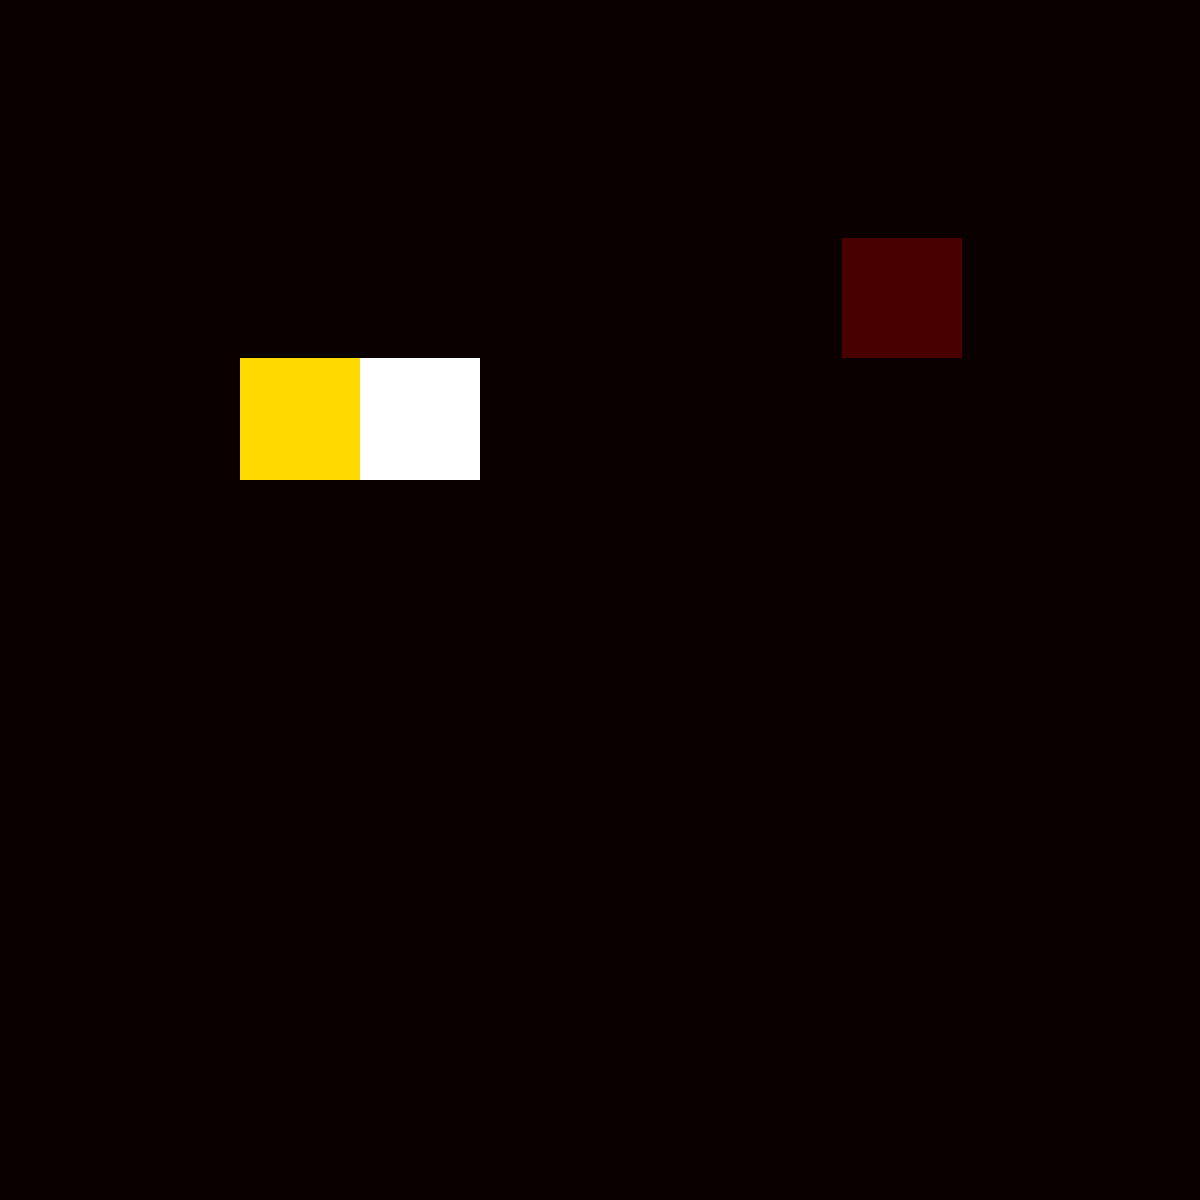
\includegraphics[width=2.4cm]{img/kamitani/encoding_2131}};
        \node (i1935) at (7, -1.3)
            {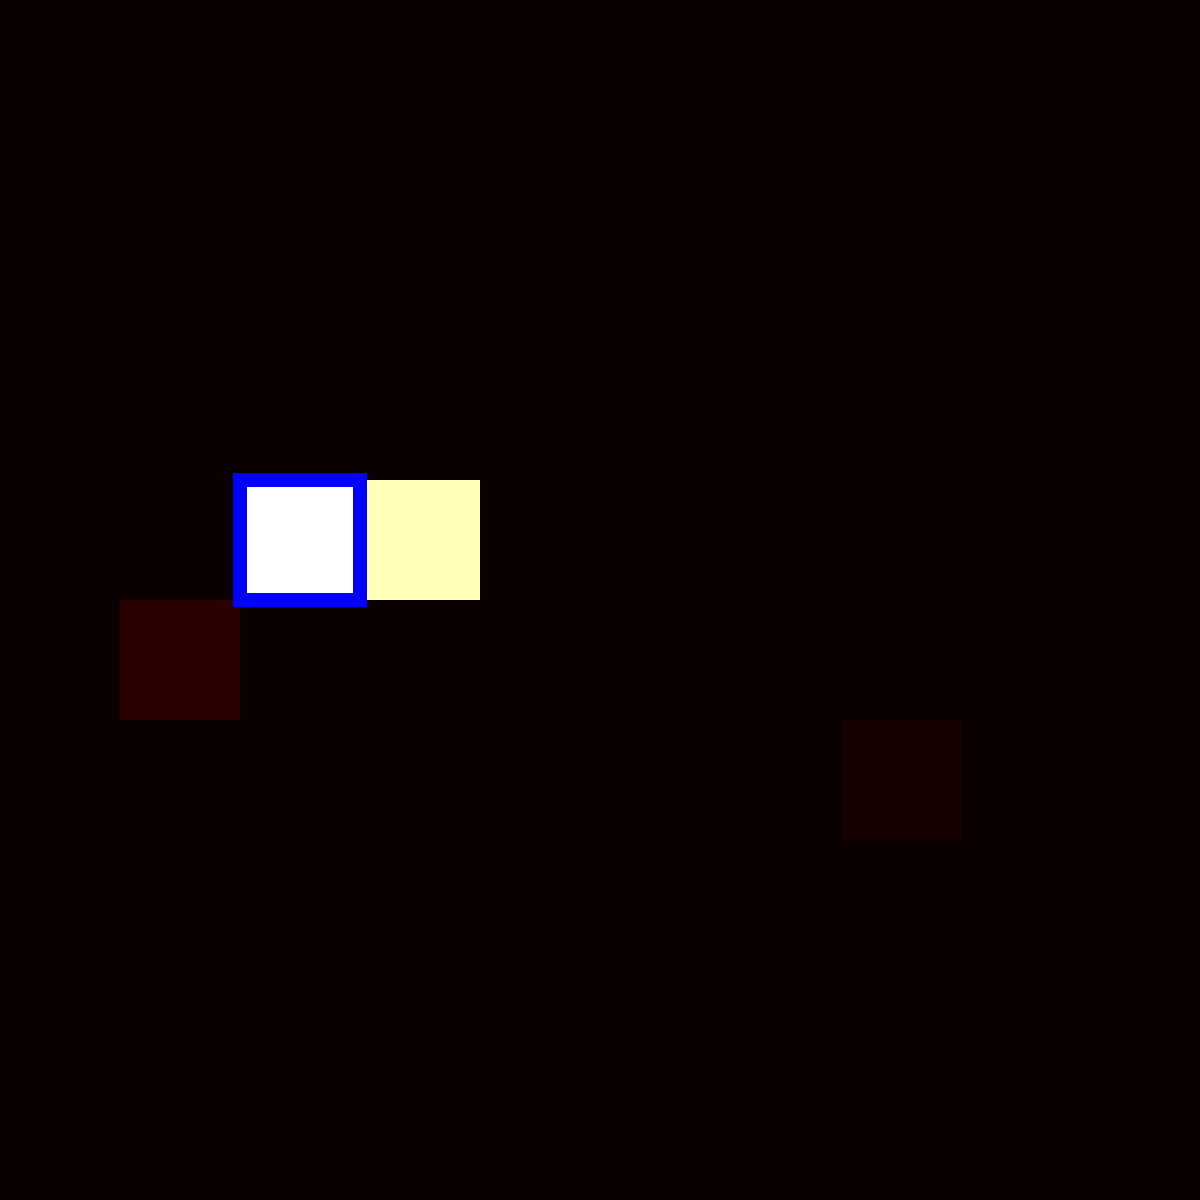
\includegraphics[width=2.4cm]{img/kamitani/encoding_1935}};

    \end{tikzpicture}
  \end{center}
  \caption{Left: reconstruction accuracy depending on pixel
           position in the stimulus. Right: receptive fields corresponding to
       voxels with highest scores and neighbours.}
  \label{fig:encoding}
\end{figure}

\section{Functional Connectivity}

\cite{biswal1995} exhibits coherent patterns in
brain activation during resting state. These correlated voxel activations are
organized in functional networks consistent with neuroscientific knowledge.

% Resting-state fMRI is useful when dealing with subjects that cannot execute a
% specific task. In fact, no task-driven protocol is capable of diagnosing precisely
% damaged brain areas e.g. in stroke patients, as no task can highlight these problems.
% \cite{varoquaux2010b} found differences in correlation between functional
% networks between control and post-stroke patients.

Here we use a dataset containing control and ADHD
(Attention Disorder Hyperactivity Disorder) patients
resting state data (subjects are scanned without giving them any specific task
to capture the cerebral background activity).

As resting state fMRI are unlabeled data, unsupervised methods must be used to
mine them. These methods group similar voxels together by comparing their time
series.
The most popular method to extract functional networks is ICA and
is the subject of our first use case. We will then show results obtained with
clustering methods as several efficient implementations are available in
scikit-learn.

The main problem with functional connectivity (and unsupervised methods in
general) is the lack of labels or ground truth. It is therefore very difficult
to score the computed models and cross validate them. A first approach is to
validate results thanks to prior knowledge, obtained in task-driven experiments
for example. Another way is to compare to functional atlases that have already
been released \citep{craddock2011,yeo2011}, the problem being that these atlases
do not agree on the number
and position of many function brain areas.

\subsection{Independent Component Analysis (ICA)}

\subsubsection{Principle}

ICA is a blind source separation method. Its principle is to separate a
multivariate signal into several components by maximizing their non-gaussianity.
A typical example is the \emph{cocktail party problem} where ICA is able to separate
voices from several people using signal from microphones located across the room.

ICA is the reference method to extract networks from resting state
fMRI \citep{kiviniemi2003}. Several strategies have been used to syndicate ICA
results across several subjects. \cite{calhoun2001a} propose a dimension
reduction (using PCA) followed by a concatenation of timeseries (used in this
example). \cite{varoquaux2010} use dimension reduction and canonical correlation analysis
to aggregate subject data. Melodic, ICA program from the FSL suite uses a Tensor
ICA approach which is not detailed here.

\subsubsection{Application}

We detrend the time series because
FastICA does not look for linear trends, only constant one.

Applying the scikit-learn ICA is straightforward thanks to the transformer
concept. As for clustering methods, a transposition of our data is required to
operate on the spatial dimension (and not on time series).

\begin{lstlisting}
from sklearn.decomposition import FastICA
X = np.vstack(Xs)
ica = FastICA(n_components=20)
components_masked = ica.fit_transform(data_masked.T).T
\end{lstlisting}

After computation, normalization and thresholding of the map is necessary to
obtain brain networks.

\subsubsection{Results}

Classical spatial ICA is compared to other evoked methods (CanICA and MELODIC).
We focus here on the default mode network because it is commonly used to
validate ICA results.

\begin{figure}[hbtp]
  \begin{center}
      \begin{subfigure}[b]{.3\linewidth}
        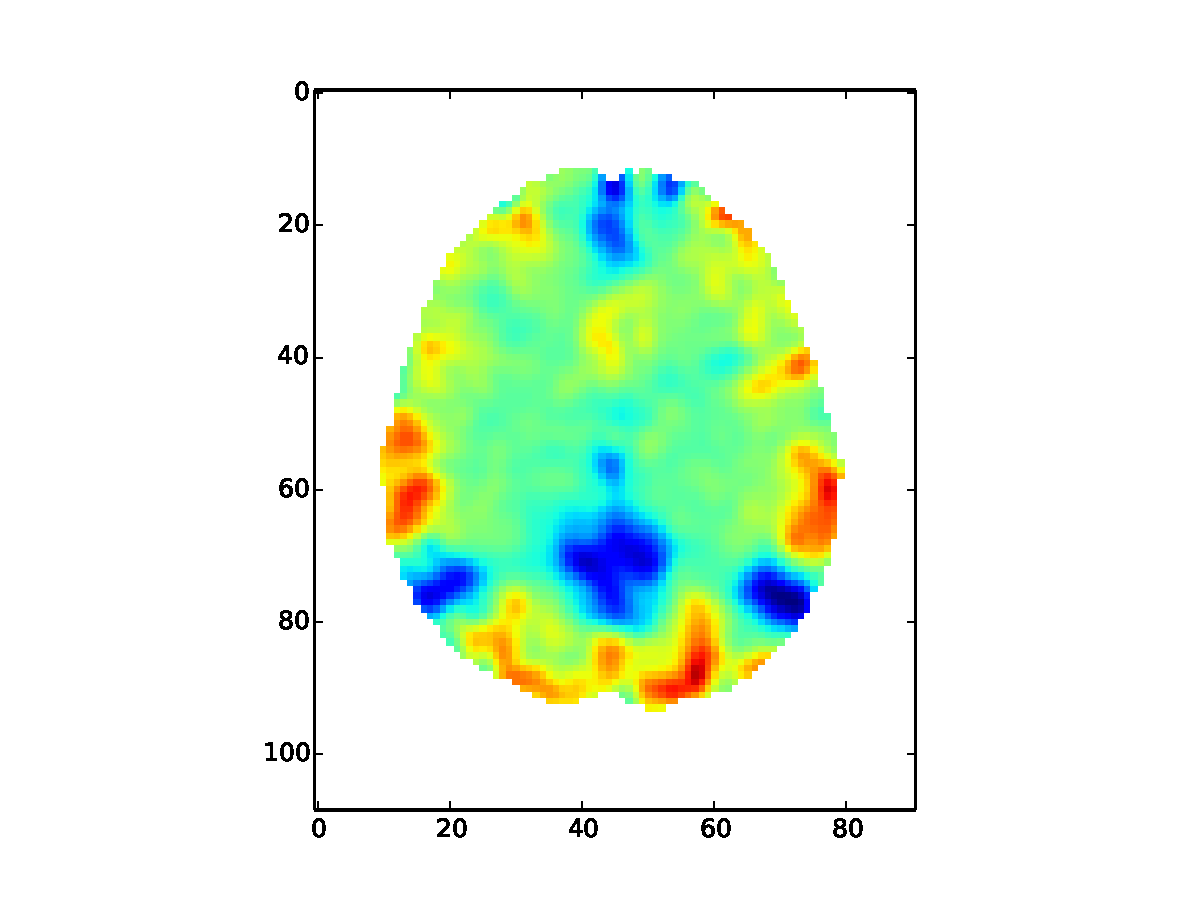
\includegraphics[width=\linewidth]{img/ica/ica}
        \caption{ICA}
      \end{subfigure}
      \begin{subfigure}[b]{.3\linewidth}
        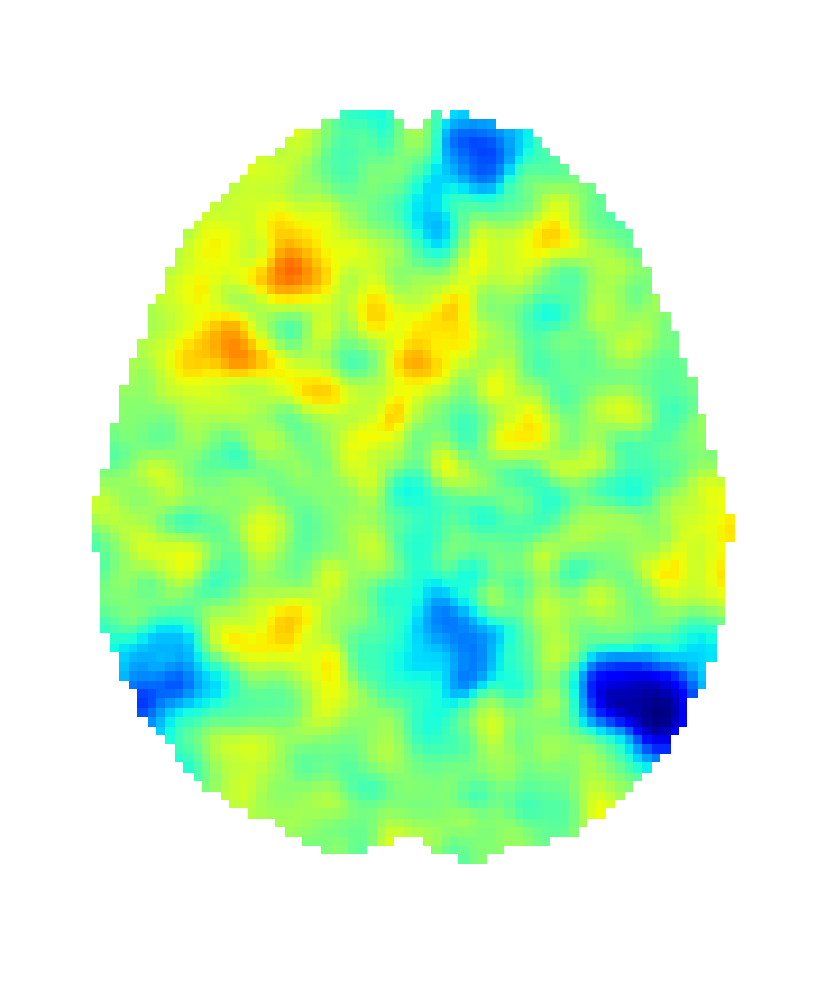
\includegraphics[width=\linewidth]{img/ica/canica}
        \caption{CanICA}
      \end{subfigure}
      \begin{subfigure}[b]{.3\linewidth}
        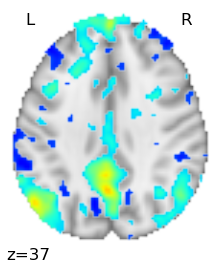
\includegraphics[width=\linewidth]{img/ica/melodic}
        \caption{melodic}
      \end{subfigure}
  \end{center}
  \caption{Extraction of default mode network using different approches}
  \label{fig:ica}
\end{figure}

\alex{After taking a closer look, it is very difficult to measure computation
time as canica and melodic are interlaced with data loading and preprocessing.}

\subsection{Clustering}
\label{clustering}

A clustering method aggregates samples into groups (called clusters) based on a similarity
measure. Unlike pure statistical methods, some clustering approaches make use of
spatial information, which is relevant in our case as we are looking for blobs.

\subsubsection{Preserving structural information}

In scikit-learn, structural information is stored apart from the data matrix
into a graph. \verb!sklearn.feature_extraction.image! provides two methods
that build an adjacency matrix based upon your data while taking the mask
into account:
\begin{itemize}
    \item \verb!grid_to_graph! creates a binary adjacency graph based upon the
        data shape; it is used in Ward's clustering.
    \item \verb!image_to_graph! creates a distance matrix using the gradient of
        the image which is used in spectral clustering.
\end{itemize}

\subsubsection{Approaches}

Several clustering approaches exists, each one having its own pros and cons.
The common parameter to all approaches is the number of clusters to extract.
Setting this parameter is not easy as we have no information about the real
number of clusters in our data (ie functional regions in the brain).

There are several ways to cross-validate this parameter (using signal variance
explained by the model for example) but this is not the subject of this paper.
In this use case, we present several clustering methods and focus on their
ability to segment well known anatomical features such as CerebroSpinal Fluid
(CSF), and amygdala.

Chosen approached are:
\begin{itemize}
    \item{\bf Ward's clustering} uses a bottom-up hierarchical approach. Features are
        progressively aggregated into clusters until a whole tree is built. This
        tree is then cut to get the requested number of clusters.
    \item{\bf k-means} is a centroid based approach. Clusters are represented by
        a central vector: a feature belongs to the cluster of the nearest
        centroid. This algorithm gives better results when data is smoothed.
% Too long to compute
%    \item{\bf spectral clustering} is a graph based approach. It separates
%        the feature graph into subgraphs by maximizing intra-group connectivity and
%        minimizing inter-group connectivity.
\end{itemize}

Common preprocessing are applied, along with a PCA to reduce dimensionality and
smoothing to enhance k-means result. Note that clustering algorithms group
samples and that we want to group features: a transposition is needed to apply
clustering in the wanted dimension. Scikit-learn provides a
\texttt{WardAgglomeration} object that takes care of this step, this is not the
case when using K-Means.

\begin{lstlisting}
connectivity = grid_to_graph(n_x=mask.shape[0], n_y=mask.shape[1],
                             n_z=mask.shape[2], mask=mask)
ward = WardAgglomeration(n_clusters=1000, connectivity=connectivity)
ward.fit(X)
\end{lstlisting}

\subsection{Results}

Clustering results are shown in figure~\ref{fig:clustering}. Cluster colors are
random. These clustering does not contain neuroscientifc information. However,
as clustering group similar voxels together, it can be used as a compression
method more sophisticated than the simple downsampling.

\begin{figure}[hbtp]
  \begin{center}
      \begin{subfigure}[b]{.23\linewidth}
          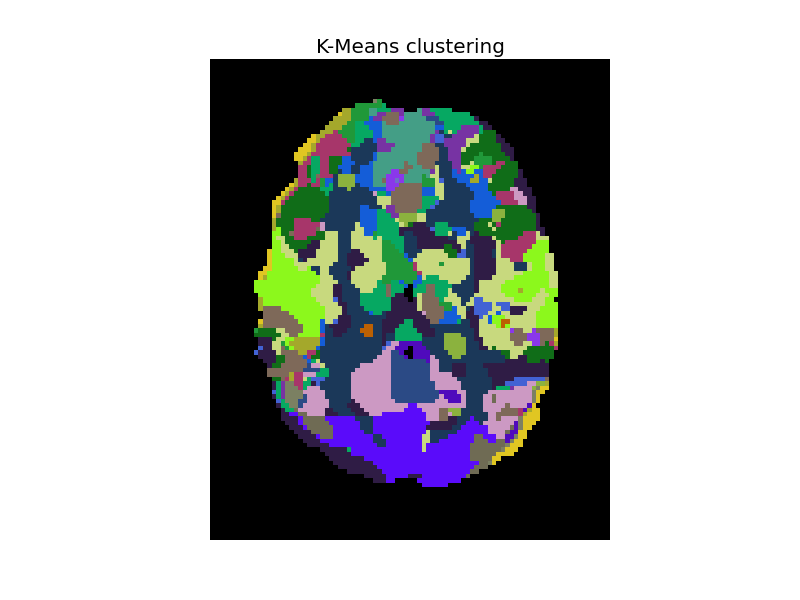
\includegraphics[width=\linewidth]{img/clustering/kmeans}
        \caption{K-Means}
      \end{subfigure}
      \begin{subfigure}[b]{.23\linewidth}
        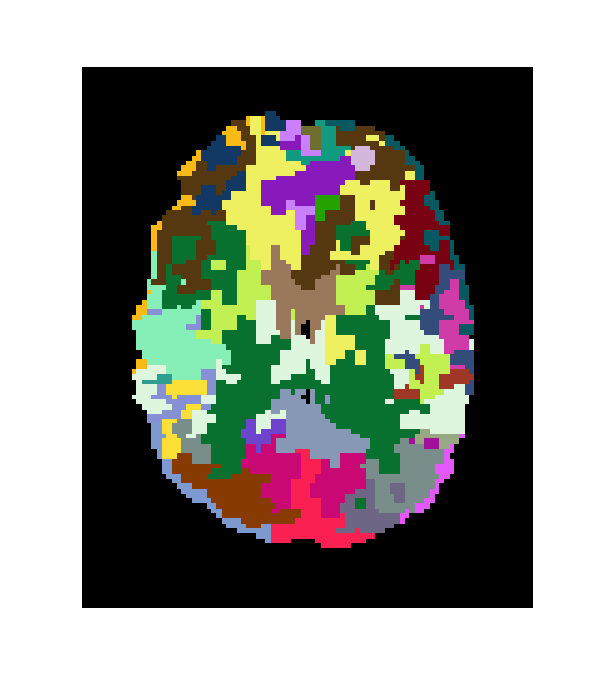
\includegraphics[width=\linewidth]{img/clustering/ward}
        \caption{Ward's clustering}
      \end{subfigure}
      \begin{subfigure}[b]{.23\linewidth}
        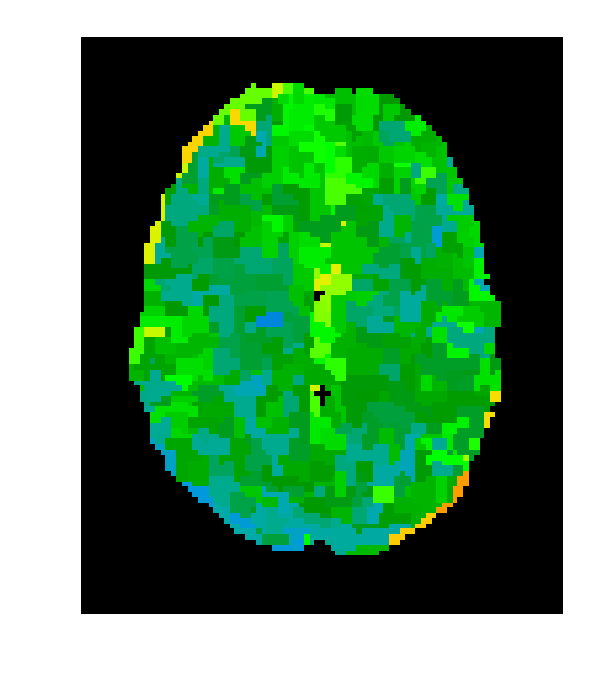
\includegraphics[width=\linewidth]{img/clustering/ward_compressed}
        \caption{Ward's compression}
      \end{subfigure}
      \begin{subfigure}[b]{.23\linewidth}
        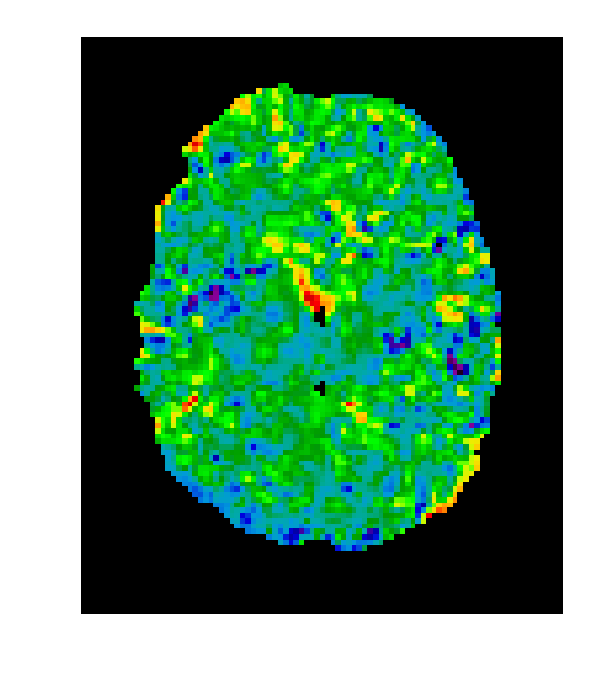
\includegraphics[width=\linewidth]{img/clustering/original}
        \caption{Original signal}
      \end{subfigure}
  \end{center}
  \caption{Brain decomposition using Ward's clustering and Kmeans. (c) shows how the original
  signal (d) is compressed using the Ward's clustering decomposition (b).}
  \label{fig:clustering}
\end{figure}

\section{Conclusion}

These use cases show that neuroscientific problems can be easily handled thanks
to scikit-learn python library. Diffculties lie in applying proper preprocessing of
the data, chosing the right model depending on the problem and interpreting
these results. An attempt to
address the first problem has been made in the nilearn Pyhton library which
provides convience tools to load neuroscientific data. However, the other
problems require skill and experience.

\section*{Disclosure/Conflict-of-Interest Statement}
%All relationships financial, commercial or otherwise that might be perceived
%by the academic community as representing a potential conflict of interest
%must be described. If no such relationship exists, authors will be asked to
%declare that the research was conducted in the absence of any commercial or
%financial relationships that could be construed as a potential conflict of
%interest.
The authors declare that the research was conducted in the absence of any
commercial or financial relationships that could be construed as a potential
conflict of interest.

\paragraph{Funding\textcolon} We acknowledge funding from the NiConnect project.

\bibliographystyle{frontiersinSCNS} % for Science articles
\bibliography{biblio}

\end{document}
